% Chapter 43: Quantum States Are Not Balls on Hidden Fixed Paths
\chapter[Quantum States and Hidden Paths]{Quantum States Are Not Balls on Hidden Fixed Paths}

Chapter 42 left a mystery: electrons, electrically steered cathode-ray specks for thirty years, diffract after passing through crystals. Diffraction is a wave signature, yet one electron always strikes a fluorescent screen as one complete point. Nobody sees half an electron. Now approach the maddening double-slit apparatus. Two narrow openings and a screen corner classical physics' deepest assumption: every object always follows a definite path, whether or not we see it.

Our task is new bookkeeping with just two rules, simple enough for one line. The price is inventing something more primitive than probability, the probability amplitude, and accepting that quantum states are not little balls secretly following fixed paths.

\step{A Counterintuitive Opening}

Modify an electron microscope so its source emits only a few thousand electrons per second while crossing the apparatus takes under one hundred-millionth of a second. At any instant its average occupancy is less than one electron. Vast temporal deserts separate electrons: they cannot meet, collide, or confer.

Place a barrier with two tiny parallel slits in front of the source and a fluorescent detector screen beyond. Each electron flashes on impact, and instruments record its position. Release them one by one.

\begin{tikzpicture}[scale=0.95,>={Stealth}]
% Electron source
\fill (0,0) circle (1.5pt) node[left=2pt]{\small Electron source};
% Double-slit barrier
\draw[thick] (3,-2) -- (3,-0.62);
\draw[thick] (3,-0.38) -- (3,0.38);
\draw[thick] (3,0.62) -- (3,2);
\node at (3.05,1.6) [right]{\small Double slit};
% Two dashed paths
\draw[dashed] (0,0) -- (3,0.5) -- (7,1.05);
\draw[dashed] (0,0) -- (3,-0.5) -- (7,1.05);
% Detector screen
\draw[thick] (7,-2) -- (7,2);
\node at (7,2.15) {\small Detector screen};
% Screen fringes; length indicates brightness
\foreach \y/\w in {-1.5/0.22,-0.75/0.62,0/0.95,0.75/0.62,1.5/0.22}
  \fill[gray!60] (7.12,\y-0.07) rectangle (7.12+\w,\y+0.07);
\node at (7.9,-1.9) [right]{\small Fringes};
\end{tikzpicture}

First electron: an apparently arbitrary dot. Second: another, far away. The first dozens resemble scattered salt without pattern. After hundreds, certain regions grow denser while others remain empty. After tens of thousands, clear alternating bright and dark stripes emerge, exactly like light's double-slit interference.

Fix on a dark band, barely visited among tens of thousands of electrons. Perform two controls. Close the right slit and leave the left: electrons now arrive there, in a bright part of the single-slit pattern. Reverse the openings: electrons arrive there too. A place accessible through either slit separately becomes inaccessible with both open.

Opening another route reduces arrivals.

Again, electrons arrive individually. Separate them by a full minute and run for months: the stripes still appear. No other electron can scout, yield, or interfere for it. Each faces both slits alone, yet its landing statistics plainly show it knows both are open.

In his physics lectures, Feynman famously called the double-slit experiment quantum mechanics' heart and only mystery: trace its other oddities far enough and they return here. This is accumulated experience, not rhetoric.

\step{Make a Guess First}

Write answers as usual and grade yourself at the end.

First: after hundreds of thousands of individually emitted electrons, do you expect two bright bands matching the slits, one smooth hump, or many alternating fringes?

Second: a dark-band location receives almost none among thousands. Close one slit: does its count (a) remain zero, (b) increase, or (c) increase but never exceed half the original?

Third, our real question: which picture describes each electron? (a) It really uses one slit, unseen by us; (b) it spreads like a cloud, half through each slit, recombining on the screen; or (c) neither?

If you chose (a), you join nearly everyone, including young Einstein. That apparently safest and most reasonable answer is precisely the most thoroughly wrong.

\step{Hands-on Experiment}

An electron double slit is unavailable at home, but two speakers can demonstrate two sources making some places quieter.

\begin{experiment}[Quiet Spots from Two Speakers]
\textbf{Materials:} two phones, or a phone and a small Bluetooth speaker; an application or webpage generating a steady tone, found by searching online sine-wave generator. Set one thousand hertz.

\textbf{Procedure:} play the same tone from both sources at equal volume, about one meter apart on a table. Cover one ear and slowly move the other sideways one or two meters before them, listening for changes. A sequence of loud--soft positions appears, some nearly silent. At one thousand hertz the wavelength is about \(34\) centimeters; neighboring quiet spots have comparable spacing, conveniently room-sized.

\textbf{Crucial step:} hold your head at a quiet spot while someone thoroughly blocks one speaker with a hand or book. What happens? Sound returns. Remove the obstruction and it fades. Adding a source quiets things; removing one makes them louder, the opening dark band's story again.

\textbf{Why:} sound consists of pressure fluctuations that add where waves overlap. If one compresses while the other rarefies, their changes cancel and the ear hears little. Cancellation depends on arriving rhythms, their phase difference, set by path difference. Integer wavelengths give synchrony and loudness; half a wavelength gives opposition and quiet.

\textbf{Think:} where did missing sound go? Nowhere: bright regions are brighter than with one source. Energy redistributes from dark to bright without changing the total. Remember this conservation for electrons later.
\end{experiment}

The analogy matches two contributions adding, reinforcing in phase and canceling out of phase. Its boundary is equally important: a microphone directly measures sound's real pressure amplitude, whereas no instrument measures the electron amplitude itself introduced below. Carry that distinction onward.

\step{The Old Model Runs into Trouble}

Pin three experimental facts to the wall, nonnegotiable for any model:

\begin{itemize}[leftmargin=1.8em]
\item Detection is whole: one flash is one point, each electron's charge, mass, and energy a complete portion, never simultaneous halves in two places.
\item Accumulated positions form alternating interference fringes.
\item Particle count does not matter: however long the gaps between individual electrons, fringes persist; each does this independently.
\end{itemize}

Now try three candidates.

\textbf{Model one: a little ball through one slit.} At any screen position it must arrive through left or right, so the distribution should sum the separate distributions, at most two overlapping humps. Fringes, especially darkness where either opening alone permits arrival, cannot appear. Failure. Perhaps collisions between electrons make fringes? Individual emission tears away that patch: with only one electron throughout, what can it collide with?

\textbf{Model two: a little wave dividing between slits.} Two waves interfere and explain stripes, but violate the first fact. Actual splitting should occasionally flash twice with half-charge at each point, or two detectors behind the slits should often each record half. Experiments say never: a full point, full charge, full click. Electrons never divide in detection. Failure again.

\textbf{Model three: one slit each time, merely unknown; left or right is probabilistic.} This common intuitive answer deserves its own trial. A concealed coin has a definite face despite your ignorance; probability records what you do not know. Then probability theory demands total arrival probability equal left-route plus right-route probability:
\[
P_{12}(x) = P_1(x) + P_2(x).
\]
No alternative exists: left and right are exhaustive and exclusive. Yet in dark bands, \(P_1 > 0\), \(P_2 > 0\), and \(P_{12} = 0\). Two positives sum to zero: probability addition receives its death sentence. If ignorance of a definite slit cannot rescue us, only abandoning a definite path at every instant remains.

All three die, but their failures indicate survival. Model three requires something cancelable, unlike nonnegative probabilities. Model two forbids a directly measured substance: the electron itself does not spread. Model one demands response to every possible path, even without something really traveling along it.

\step{Inventing New Concepts}

Feynman historically organized the new language most cleanly. Three rules suffice:

\textbf{Rule one: assign an arrow to every indistinguishable alternative.} An electron can reach a screen point through left or right. If no apparatus or record can distinguish those alternatives even in principle, draw an arrow for each. It has length and direction: probability amplitude, whose direction is called phase.

\textbf{Rule two: indistinguishable alternatives add arrows.} Join arrows tip to tail and connect start to finish, exactly planar displacement-vector addition. Phase now matters: matching directions maximize the sum, opposite directions shrink it to a point, and intermediate angles give intermediate lengths. This is superposition: quantum states add as arrows, not numbers.

\textbf{Rule three: probability is the resultant length squared.} This is the Born rule. Direction alone does not affect probability; it matters only when arrows combine. The observable world, whether a screen flashes, sees length alone; phase stays backstage, appearing indirectly through addition.

Generalize to our protagonist. Assign each possible detection position \(x\) an arrow \(\psi(x)\), the wavefunction. Squared length of \(\psi(x)\) gives detection probability near \(x\), strictly probability density. Screen, slit, and intermediate points each have arrows; together they constitute the electron's quantum state across the apparatus. This is no inventory of hiding places but a complete answer to what any measurement can yield and with what probability.

Now solemnly separate three things popular accounts often stew together.

\textbf{Experimental facts}: individual dots, accumulated stripes, and dark bands brightening when a slit closes. They do not depend on theory and are reproducible.

\textbf{Mathematical model}: arrows, addition, squared modulus, and \(\psi(x)\). These invented calculation rules earn their place solely by point-by-point agreement between predicted probabilities and experiment.

\textbf{Physical interpretation}: what are arrows? Does a wavefunction exist physically or merely record accounts? Does an electron have a position before measurement? The rules explain none of this; they specify calculation, not the world's internal play. Physicists have argued for a century, writing different scripts with identical probabilities. Chapter 45 maps interpretations. Here keep one discipline: never preach a script as experimental fact.

Revisit our three recurring questions. What is the system's present state? Mechanics gives positions and momenta; heat gives macroscopic parameters; quantum mechanics gives a state, amplitudes sufficient to compute every measurement's probabilities. What law changes that state? Chapter 44's Schrödinger equation. How do measurements reveal it? The Born rule and Chapter 45's measurement process. The old questions remain; their answers acquire new grammar.

Finally complete the amplitude analogy. Like water-wave height, it superposes and cancels crest against trough to make interference. Unlike water height, it is not directly measurable substance: it can be negative and needs two numbers, as shortly shown. Asking its value here has no operational meaning; you can only count electron arrivals. It mediates probability calculation, is not probability itself, and is certainly no diluted material wave.

\step{The Model in One Sentence}

\begin{oneline}
Every indistinguishable path contributes a phase-bearing arrow; add arrows first and square the resultant length for probability. A quantum state is no ball secretly following a fixed path: without a record, which path has no answer.
\end{oneline}

\step{The Mathematical Translator}

Write the rules mathematically and test extremes immediately.

\textbf{First: add amplitudes, square for probability.} For paths with \(A_1\) and \(A_2\),
\[
A = A_1 + A_2, \qquad P = |A|^2.
\]
Bars mean arrow length. Test two equal arrows of length \(a\). In phase: length \(2a\), probability \(4a^2\), four times each separate \(a^2\), not twice. A bright fringe with both slits is twice the sum of separate contributions, the extra brightness supplied by darkness elsewhere. Opposite: arrows face head-to-head, resultant zero, \(P = 0\). Two possible arrivals yield certain nonarrival, impossible with probabilities but immediate with amplitudes. Perpendicular: Pythagoras gives \(\sqrt{2}\,a\) and \(2a^2\), the separate-probability sum. Classical \(P = P_1 + P_2\) is not wrong but the ninety-degree-phase special case, a projection of a more general rule rather than an axiom.

\begin{tikzpicture}[>={Stealth},scale=1.05]
% Same phase
\draw[->,thick] (0,0) -- (1,0);
\draw[->,thick] (1,0) -- (2,0);
\draw[->,very thick] (0,-0.45) -- (2,-0.45);
\node at (1,-0.95) {\small \shortstack{In phase: length \(2a\),\\\(P=4a^2\)}};
% Opposite phase
\draw[->,thick] (4,0) -- (5,0);
\draw[->,thick] (5,0) -- (4,0);
\fill (4,-0.45) circle (1.2pt);
\node at (4.5,-0.95) {\small \shortstack{Opposite: length \(0\),\\\(P=0\)}};
% Perpendicular
\draw[->,thick] (8,0) -- (9,0);
\draw[->,thick] (9,0) -- (9,1);
\draw[->,very thick,dashed] (8,0) -- (9,1);
\node at (8.75,-0.95) {\small \shortstack{Perpendicular:\\length \(\sqrt{2}\,a\), \(P=2a^2\)}};
\end{tikzpicture}

\textbf{Second: where the fringes lie.} In double slits, phase differences mainly come from path differences. Chapter 42 gives wavelength \(\lambda = h/p\); an extra \(\Delta s\) gives
\[
\Delta\varphi = \frac{2\pi\,\Delta s}{\lambda}.
\]
In-phase paths, \(\Delta s = 0, \lambda, 2\lambda, \dots\), are brightest; opposite paths, \(\Delta s = \lambda/2, 3\lambda/2, \dots\), are dark. Geometry gives neighboring bright-fringe spacing
\[
\Delta y = \frac{\lambda L}{d},
\]
where \(d\) separates slits and \(L\) separates barrier and screen. Doubling \(L\) or \(\lambda\) doubles spacing: longer waves or farther screens spread patterns. Doubling \(d\) halves it: wider slit separation crowds fringes. As \(\lambda \to 0\), \(\Delta y \to 0\); unresolved dense stripes resemble a smooth hump. Remember this limit for baseball interference's invisibility.

\textbf{A real-data estimate: fringe width.} Electrons accelerated through one hundred volts have Chapter 42's momentum \(5.4\times10^{-24}\,\mathrm{kg\cdot m/s}\) and wavelength \(\lambda \approx 0.12\,\mathrm{nm}\). Choose \(d = 100\,\mathrm{nm}\), roughly virus-sized, and \(L = 10\,\mathrm{cm}\):
\[
\Delta y = \frac{1.2\times10^{-10}\times0.1}{1.0\times10^{-7}} \approx 1.2\times10^{-4}\,\mathrm{m}.
\]
Order one-tenth millimeter. Electron fringes do not visibly cover a wall but appear clearly under electron-microscope magnification. That is how the opening image of tens of thousands of electrons weaving fringes was made, with Tonomura's team producing a textbook version around 1989. The estimate exposes the difficulty: \(d\) must be nanometric and the slits narrower still. Enlarge any dimension a hundredfold and fringes blur together.

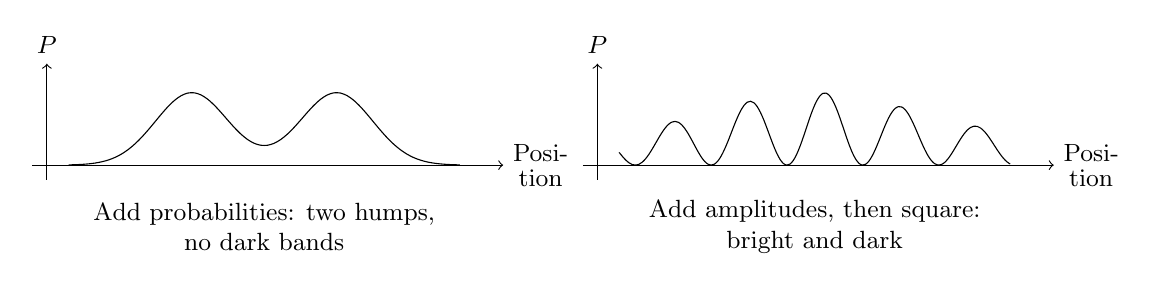
\begin{tikzpicture}[scale=0.92]
% Left: adding probabilities
\draw[->] (-0.2,0) -- (6.3,0) node[right]{\small \shortstack{Posi-\\tion}};
\draw[->] (0,-0.2) -- (0,1.4) node[above]{\small \(P\)};
\draw[domain=0.3:5.7,samples=60,smooth] plot (\x,{exp(-((\x-2.0)^2)/0.5)+exp(-((\x-4.0)^2)/0.5)});
\node at (3,-0.85) {\small \shortstack{Add probabilities: two humps,\\no dark bands}};
% Right: adding amplitudes, then squaring
\begin{scope}[xshift=7.6cm]
\draw[->] (-0.2,0) -- (6.3,0) node[right]{\small \shortstack{Posi-\\tion}};
\draw[->] (0,-0.2) -- (0,1.4) node[above]{\small \(P\)};
\draw[domain=0.3:5.7,samples=120,smooth] plot (\x,{0.5*(1+cos(6*\x r))*(0.35+0.65*exp(-((\x-3.0)^2)/4))});
\node at (3,-0.85) {\small \shortstack{Add amplitudes, then square:\\bright and dark}};
\end{scope}
\end{tikzpicture}

\textbf{Third: why arrows need two numbers, introducing complex numbers.} A planar arrow needs horizontal and vertical components. Mathematics already names paired numbers with arrow addition: complex numbers. Horizontal \(a\), vertical \(b\), gives \(a + bi\), where \(i\) has one definition: multiplying by \(i\) means rotating ninety degrees counterclockwise. Twice gives \(i \times i = -1\), complete reversal, the famous \(i^2 = -1\). No mysticism, just two right-angle turns. Phase is rotation, and complex multiplication automatically combines rotations: multiply two numbers instead of learning a new mnemonic. Real numbers offer only a negative sign, same or opposite directions, nowhere for continuously varying ninety- or thirty-seven-degree phases. Complex numbers are not affectation but the native language of arrows and rotations. Nor does imaginary mean unreal, any more than negative accounts make debt fictional. Measured squared moduli are thoroughly real counts.

\begin{mathbridge}
\textbf{Expand the square to expose interference.} Amplitude magnitudes are \(|A_1| = a_1\) and \(|A_2| = a_2\), separated by \(\Delta\varphi\). Vector lengths, or the cosine rule, give
\[
P = |A_1 + A_2|^2 = a_1^2 + a_2^2 + 2a_1a_2\cos\Delta\varphi
   = P_1 + P_2 + 2\sqrt{P_1P_2}\cos\Delta\varphi.
\]
The first two terms add classical probabilities; the third is interference, quantum theory's extra column. Check \(\Delta\varphi = 0\): \(\cos = 1\), \(P = (\sqrt{P_1}+\sqrt{P_2})^2\), constructive and bright. For \(\Delta\varphi = \pi\): \(\cos = -1\), \(P = (\sqrt{P_1}-\sqrt{P_2})^2\), zero for equal paths, dark. For \(\Delta\varphi = \pi/2\), interference vanishes and classical addition returns. Most interestingly, if phases fluctuate irregularly, time or ensemble averaging makes positive and negative \(\cos\Delta\varphi\) cancel to zero. Interference evaporates and probability addition revives. Remember that zero average: Chapter 45 shows how environmental phase scrambling largely makes the macroscopic world classical.

In complex notation, \(A = a + bi\) has \(|A|^2 = a^2 + b^2\). A unit arrow at \(\theta\) is \(A = \cos\theta + i\sin\theta\). Wavefunction normalization requires
\[
\int |\psi(x)|^2 \, dx = 1,
\]
meaning the electron must be detected somewhere and all position probabilities sum to one. Bookkeeping forbids particles appearing from nowhere.
\end{mathbridge}

\begin{challenge}
\textbf{Why probabilities alone fail, and how arrows rotate in time.}

Suppose someone insists on probabilities alone. Each position receives a nonnegative number and path contributions only add. Nonnegative plus nonnegative cannot cancel. Allowing cancellation requires negative contributions; continuously tunable cancellation requires a continuously varying angle. Amplitudes are the smallest experimentally forced upgrade, with no simpler alternative.

What does the arrow do between measurements? Chapter 42 associates energy \(E\) with \(f = E/h\). Precisely, a fixed-length arrow rotates uniformly at angular speed
\[
\omega = \frac{E}{\hbar}, \qquad \hbar = \frac{h}{2\pi} \approx 1.05\times10^{-34}\,\mathrm{J\cdot s}
\]
Its amplitude multiplies over time by \(\cos\omega t + i\sin\omega t\), compactly \(e^{i\omega t}\) via Euler's formula. Overall rotation of one arrow is unmeasurable because Born sees only length. Two path arrows rotating at different rates instead develop relative phase drift and moving fringes. Energy differences are phase-rotation-rate differences. The law governing those rotations in each situation is a dynamical equation, Schrödinger's, Chapter 44's protagonist. Our addition and squaring rules are its admission ticket.
\end{challenge}

\step{The Model's Limits}

This powerful language carries the following scope and authenticity labels.

First, wavefunctions predict, not constitute material clouds. Large \(|\psi(x)|^2\) means high detection probability here, not part of an electron spread here. Detection always gives one full particle and point. What spreads in the opening image is thousands of independent events' statistical distribution, not any electron's shape.

Second, amplitude is not probability. Negative or complex, cancelable by another arrow, it has no probability-of-occurrence interpretation. No instrument anywhere directly reads \(\psi(x)\), only count rates proportional to squared modulus. Mistaking amplitude for finer-grained probability is the first beginner trap.

Third, quantum probability is not ignorance. A hidden coin has a definite answer; an unrecorded electron path has no answer at all. Dark bands prove it: definite paths would preserve probability addition. This also marks classical territory: distinguishable paths, for example recorded by apparatus, erase interference and revive probability addition, making balls useful again. Chapter 45 explains what happens; here mark the boundary.

Fourth, electrons do not alternate between wave and particle forms. They always admit amplitude descriptions and whole-point detections. The borrowed macroscopic words each capture half, and alternating them falsely suggests costume changes.

Fifth, why do macroscopic things look so ball-like? Two reasons. Short wavelength: a \(0.2\,\mathrm{kg}\) baseball at \(20\,\mathrm{m/s}\) has \(\lambda = h/(mv) \approx 1.7\times10^{-34}\,\mathrm{m}\). From \(\Delta y = \lambda L/d\), fringes are twenty orders tighter than nuclei; detectors see only averaged smoothness. Fragile phase: countless photons and air molecules collide with its surface each second, objectively recording position and scrambling phases until interference averages away, precisely the bridge's zero-average \(\cos\) mechanism. Secret fixed-path balls are therefore a vast-domain macroscopic approximation, not simply a wrong theory. Double slits stand at its boundary.

Sixth, common misuses: superposition makes macroscopic objects simultaneously available in two places, false by the fifth point; electrons have unknown definite premeasurement positions, false by model three's dark-band verdict; amplitudes are psychological probabilities or subjective beliefs, false because they are objective law-governed quantities; many electrons collectively make fringes, false because individual emission reproduces them.

\step{Explaining the Opening Phenomenon}

Return to the apparatus and close each mystery.

Why individual points? An arrival is a detection event, and Born gives its position probability. The event itself is whole: an instrument clicks or does not, never half-clicks. Points speak measurement's language.

Why do points weave stripes? Without any path record, each electron's two paths contribute amplitudes, added and squared at every position. The resulting probability landscape has peaks and valleys; independent arrivals reveal fringes automatically. Electrons do not arrange stripes; they follow probability's mountains and chasms.

Why does closing one slit brighten darkness? Equal opposite amplitudes cancel there. It is not inaccessible: two contributions oppose. Removing one arrow leaves a nonzero probability and arrivals. Supernatural under probability addition, ordinary vector arithmetic under amplitude addition.

Why fringes even a minute per electron? Each interferes through its own two amplitudes, independently of every other electron. It completes the whole experiment alone with its own arrows. Colliding, negotiating, relaying electrons have no partners even in principle.

Where did missing dark-band electrons go? Into brightness. Bright-center probability is four times a single contribution, not twice, the excess supplied by dark bands; all probabilities always sum to one. As missing sound reappears elsewhere louder, phase redistributes energy's address without destroying it.

These split--phase--recombine rules are engineering tools now. Atom interferometers separate and reunite whole-atom wave packets. Tiny gravitational-acceleration changes produce measurable relative phases, so fringe motion reads gravity. The best atomic gravimeters detect billionth-level changes, exploring underground deposits and voids and providing satellite-free submarine inertial navigation. Our three rules supply their entire operating principle.

Complete the speaker analogy's boundary too. Like double slits, contributions reinforce or cancel by phase and blocking one revives darkness. Unlike them, sound amplitude is directly measurable air pressure requiring a medium. Electron amplitude is unmeasurable and medium-free, not a ripple in substance. Beyond that boundary analogy misleads.

Daily noise-canceling headphones use the same opposing-phase idea. Microphones sample outside noise while speakers emit real-time opposite waves, reducing pressure fluctuations at the eardrum. This classical interference is the speaker experiment's quiet spot. Again the distinction: pressure is a directly measurable real quantity and oscilloscopes display its arrows, whereas nobody sees electron amplitudes.

An easily missed fact: photons obey the same rules. Single-photon double slits reproduce each line of the script, individual points, accumulated fringes, and darkness brightened by closure. The familiar Mach--Zehnder interferometer is a photon double slit: a beam splitter separates two routes, reunited after different distances, with phase-dependent detector counts. Electrons, photons, atoms, and carbon-sixty molecules share one ledger. That is why we say quantum rather than electron state: universal rules, changing actors.

\step{Thought Experiments and Challenges}

\begin{thought}[Enlarging Double Slits from Electrons to You]
What larger things interfere? These are no longer just imagined experiments but a real sequence up the size scale.

In 1999, Zeilinger's team sent carbon-sixty molecules, sixty-atom soccer balls weighing about \(1.2\times10^{-24}\,\mathrm{kg}\), over a million electron masses, at roughly two hundred meters per second through a \(100\,\mathrm{nm}\)-period grating. Their \(\lambda = h/(mv) \approx 2.8\times10^{-12}\,\mathrm{m}\), about three picometers, is tens of times smaller than atoms. Estimating \(\lambda L/d\) gives characteristic spacing of tens of micrometers, and experiment genuinely resolved diffraction. A sixty-atom ball vibrating with internal heat still refuses a fixed path.

Enlarge to the baseball with \(\lambda \approx 1.7\times10^{-34}\,\mathrm{m}\). Visible fringes require slit separation order \(10^{-30}\) meters, over ten thousand times smaller than a nucleus, and no information exchange with even one photon or air molecule throughout flight. The latter seals its fate: the environment measures it every instant, path records abound, and interference is already averaged away.

The analogy resembles a zooming-out camera showing no wall between quantum and classical, only a gradient: shorter wavelengths, less enduring phases, increasingly accurate balls. It is not an engineering blueprint. Carefully cooling a baseball cannot reveal its interference because environmental records close that route in principle. Classicality is macroscopic fate, not insufficient technology.
\end{thought}

\begin{puzzles}
\item Halve one speaker's volume. Do quiet spots remain entirely silent? \textbf{Hint:} what conditions permit complete cancellation? Add unequal opposite arrows. What resultant remains, and what replaces silence?
\item Increase electron acceleration voltage in the double slit. Do faster electrons produce wider or narrower fringes? \textbf{Hint:} track momentum and \(\lambda = h/p\), then substitute into \(\Delta y = \lambda L/d\). Why were electron-interference experiments historically harder than optical ones?
\item Blindfold yourself and randomly send a glass ball through one slit per trial. Why do ten thousand trials give only two \(P_1 + P_2\) humps, unlike electrons' dark bands? \textbf{Hint:} does blindfolding change knowledge or the existence of records? Do air collisions, reflected sound, or brushed dust record the route? Is a two-path amplitude phase operationally meaningful for the ball?
\item Someone claims sufficiently good instruments always directly measure local amplitude magnitude and phase. Refute this. \textbf{Hint:} what events underlie every signal you create and read? Is each detector response a continuous arrow reading or a complete count? Which amplitude property determines count rate? Why are relative phases measurable, and what role does fringe displacement play?
\end{puzzles}

We have delivered a prediction machine: state, amplitudes for indistinguishable paths, addition, squaring, probabilities. It predicts present measurements but remains silent on how the state evolves between them. What law rotates the phase arrow? An equation is needed, just as Newton supplied one for changing motion. Chapter 44 provides Schrödinger's; Chapter 45 reserves the deeper measurement story.
